\chapter{Retrospective dedicated games}
Communication inside any team can be difficult especially when it involves revealing your own personal opinion which might differ from others. Speaking out loud about problems even in small group might be shameful and most of people do not like to open up in front of others, which might cause layering issues not only in communication between people, but also in developing good quality software. Based on experience that we learned from Scrum Masters and Technical Leaders in company Intel Technology Poland, most people have enormous knowledge about technology, new frameworks or developing with good standards, but they are not used to share it, because they are afraid of criticism, so they rather sit quiet and let other, more brave, sometimes less experience, people talk. 
The following games are invented for the situations, which were mentioned before to minimize the shyness and fear and to maximize awareness of possible problems and to enforce team to discuss them.

\section{Fundamental games}
\label{s:fundGames}
To start with, we should be aware of existence of a standard procedure mentioned in \autoref{chap:meetingsOverview}. The 3-statement method which contains "Good things", "Bad things" and "Things to improve" is the most popular and the most frequently used by teams, based on Grzegorz Regliński knowledge and experience, technique of conducting Retrospective. Games presented in this chapter are an innovative approach to this meeting, which often changes users' point of view, shows a problem, both inside and outside of the team, from a different angle and entertains, while retrieving interesting and impressive results. 

\subsection{Speedboat game}
\label{subch:speedboatGame}
“Speedboat” (also known as Sailboat) is a game which changes the perspective of looking on retrospective and problems. Team members do not focus what problems they had in terms of ordering them into three columns using 3-statement method, but thanks to change of view they start to think creatively and might retrieve more valuable issues. \autoref{fig:speedboat} shows what should be drawn on a blackboard. Every item represents different statement \cite{SpeedboatBibliography}:
\begin{enumerate}
    \item The cloud which is creating the wind symbolizes things that were successful, things that are pushing forward our team and product, for example good code reviews in previous sprint, members of the team share knowledge and help others.
    \item The anchor symbolizes things which could have been done better, because the idea is good but the execution is not being done well, for example crowding pull request reviews because only one person is doing them, bad communication in the team caused e.g. solving problems that someone already had and did not share with others the solution, wasted time.
    \item The rocks symbolize statement things that we wish did not happen again, something that may cause our product major problems now or in the future, those are things that we need to lose, for example planning did not go well, so many people were without tasks because of bad division or dependency.
\end{enumerate}

\begin{figure}[h]
\caption{Speedboat}
\label{fig:speedboat}
\centering
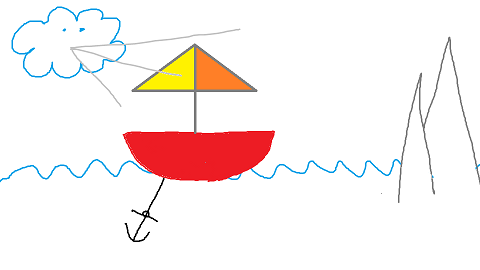
\includegraphics[width=0.5\textwidth]{img/speedboat}
\end{figure}

The game should start with describing people what is game about. The main aspect is that people understand what is required from them during “Speedboat” game. The \autoref{tab:speedboat-req} below shows what is required to start with this improvement game.

\begin{table}[h]
	\caption{Requirements to start Speedboat game}
	\label{tab:speedboat-req}
	\begin{tabularx}{\textwidth}{|X|X|}
	\hline
		Target & Improve creativity in the team and maximize solving problems  \\ \hline
		Required			& \begin{enumerate}
		    \item Minimum 3-people scrum team
		    \item Blackboard
		    \item Sticky Notes
		    \item Pencil/Pen
		\end{enumerate}	 \\ \hline
		Time			& About \~45 minutes	 \\ \hline

	\end{tabularx}
\end{table}

After description the leader draws the picture, like on  \autoref{fig:speedboat} and team members should stick sticky notes where think they belong. The next step, if everybody already is out of ideas, is to discuss the results displayed on blackboard, maybe a particular issue is for one person positive and for another is negative, they should clarify and talk about it. This approach is not only productive for the team, but also for project, and might retrieve interesting outcome.

\subsection{Glad/Mad/Sad game}
\label{subch:gmsGame}
The Glad, Mad, Sad game, also known as Happy, Sad, Angry is a game in which the manager or scrum master is able to observe teams mood, which is definitely a useful factor to retrieve from a retrospective meeting. \autoref{fig:hsapic} visualizes how the scrum master should draw in order to conduct "Happy/Sad/Angry" game. The board should be divided to three spaces, where each space has its own meaning and purpose \cite{HSABibliography}:
\begin{enumerate}
    \item Happy Face symbolizes successful things which occurred in current iteration, accomplishments and valuable effects for the team and project, things that we learned and you are thankful for.
    \item Sad Face symbolizes things that made a team member not satisfied of his/hers work, an action which could be done better.
    \item Angry Face symbolizes things which caused problems that made team members annoyed, issues which were the source of iteration failure or the work harder than could have been using e.g. other tool, framework etc.
\end{enumerate}
\begin{figure}[h]
\caption{Happy/Sad/Angry}
\label{fig:hsapic}
\centering
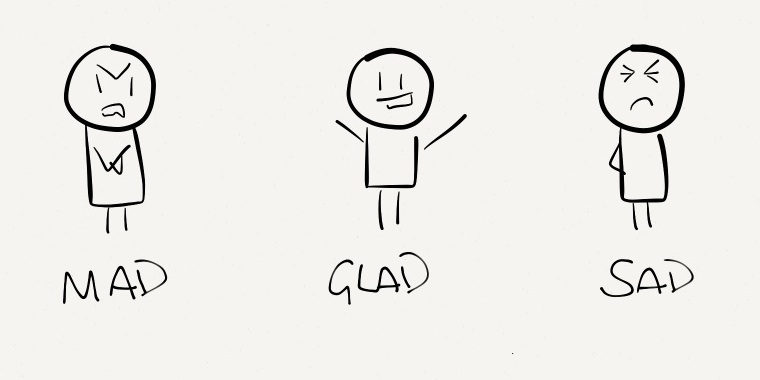
\includegraphics[width=0.5\textwidth]{img/mgs}
\end{figure}

To start with the leader, who is responsible for retrospective should describe the rules of described in this subsection game. Required equipment for this approach is presented in \autoref{tab:hsa-req}.

\begin{table}[h]
	\caption{Requirements to start Happy/Sad/Angry game}
	\label{tab:hsa-req}
	\begin{tabularx}{\textwidth}{|X|X|}
	\hline
		Target & Retrieve teams mood and maximize solving problems  \\ \hline
		Required			& \begin{enumerate}
		    \item Minimum 3-people scrum team
		    \item Blackboard
		    \item Sticky Notes
		    \item Pencil/Pen
		\end{enumerate}	 \\ \hline
		Time			& About \~45 minutes	 \\ \hline

	\end{tabularx}
\end{table}

The next steps, after team members understands what is the purpose and what are the rules of described game, are the same as in Speedboat game, filling sticky notes and discussion.

\subsection{Starfish Game}
\label{subch:starfishGame}
The next game I would like to describe shows a totally different approach for conducting retrospective. The game is called "Starfish" \cite{StarfishBibliography}, because this shape divides board to five areas like on \autoref{fig:starfish} :
\begin{enumerate}
    \item Keep doing - this area describes things which are being done well by the team and they should continue doing them because they are valuable for the project and team members.
    \item Stop doing - things which are "not bringing value, or even worse, it is getting on the way"\cite{StarfishBibliography}.
    \item Start doing - things which were working for you in the past in other team/project or new ideas, approaches which might help team in delivering product and in general are beneficial for the team.
    \item Less of - things which are being done already and they bring value, but should be reduced.
    \item More of - things which are being done already and they bring value, but they would bring more value if done more \cite{StarfishBibliography}.
\end{enumerate}

\begin{figure}[h]
\caption{Starfish}
\label{fig:starfish}
\centering
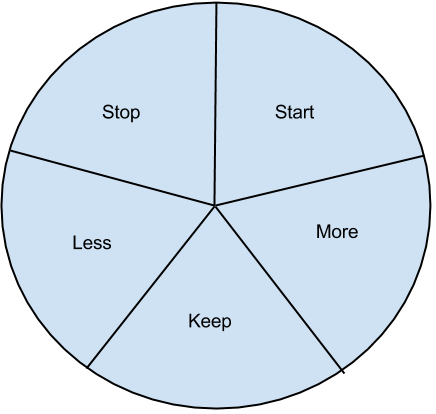
\includegraphics[width=0.5\textwidth]{img/starfish}
\end{figure}

This game shows a different perspective than is in usual 3-statement method and thanks to that, leaders are able to retrieve problems and issues in nonstandard fields. The requirements are presented in \autoref{tab:starfish-req}.

\begin{table}[h]
	\caption{Requirements to start Starfish game}
	\label{tab:starfish-req}
	\begin{tabularx}{\textwidth}{|X|X|}
	\hline
		Target & Retrieve problems, increase creativity and maximize solving problems  \\ \hline
		Required			& \begin{enumerate}
		    \item Minimum 3-people scrum team
		    \item Blackboard
		    \item Sticky Notes
		    \item Pencil/Pen
		\end{enumerate}	 \\ \hline
		Time & About \~60 minutes \\ \hline

	\end{tabularx}
\end{table}

\subsection{360-degrees of appreciation Game}
\label{subch:360Game}
Another team building game is called 360-degrees of appreciation and is an activity that fosters open appreciation feedback within a team. The game is useful in case of increasing team moral and improving people relationship. The \autoref{tab:360-req} presents requirements for the game and the rules are as follows  \cite{360Bibliography}:
\begin{enumerate}
    \item Gather all participants around the table.
    \item Write appreciations on your paper for each member of the team gathered around the table.
    \label{it:apprTabTimeWritting360}
    \item If everyone is ready, ask the participants to sit in a circle.
    \item Chose one person that will sit or stand in the middle of the circle.
    \item Everyone in the circle should read theirs appreciations toward the person sitting in the center.
    \label{it:apprTabTimeTalking360}
    \item Repeat steps four and five for everyone in the circle.
\end{enumerate}

\begin{table}[h]
	\caption{Requirements to start 360-degrees of appreciation game}
	\label{tab:360-req}
	\begin{tabularx}{\textwidth}{|X|X|}
	\hline
		Target & Motivates constant feedback, strengthens relationship and trust \\ \hline
		Required			& \begin{enumerate}
		    \item Minimum 3-people scrum team
		    \item Paper or Sticky Notes
		    \item Pencil/Pen
		\end{enumerate}	 \\ \hline
		Time			& About \~2 minutes for each participant for the \autoref{it:apprTabTimeWritting360} of rules and about \~10 minutes for \autoref{it:apprTabTimeTalking360}\\ \hline

	\end{tabularx}
\end{table}

\subsection{Mood and improvements Game}
\label{subch:moodGame}

During the cooperation with Intel Technology Poland teams, the "Mood and improvements" game has been created. The activity is a merge of two approaches, both of them were already described, first in the \autoref{subch:gmsGame} and the second one  has its roots and has been inspired by the game from \autoref{subch:360Game}. The goal is to retrieve as valuable as possible feedback from the team about the project and simultaneously increase the trust, strengthen the relationship between team members and retrieve from the team ideas how to improve the project or the team. 
As presented on \autoref{fig:moodPic} the game has five areas that need to be filled. The first three fields on the top are described in \autoref{subch:gmsGame}, because the upper part of the picture is the exact reflection of Glad, Mad, Sad game. The lower area of the \autoref{fig:moodPic} presents:
\begin{enumerate}
    \item Flowers - representation of statement "Appreciations", in this section we thank people for things that they have done for us, the team, the project in the past iteration, e.g. quick and upright code review, help in the task etc.
    \item Light bulb - is the representation of expression "Ideas", in this area we stick the papers with concepts how to improve the team or the project, e.g. estimate more carefully on the planning, dedicate some time in the iteration to increase code coverage etc.
\end{enumerate}

\begin{figure}[h]
\caption{Mood and Improvements} 
\label{fig:moodPic}
\centering
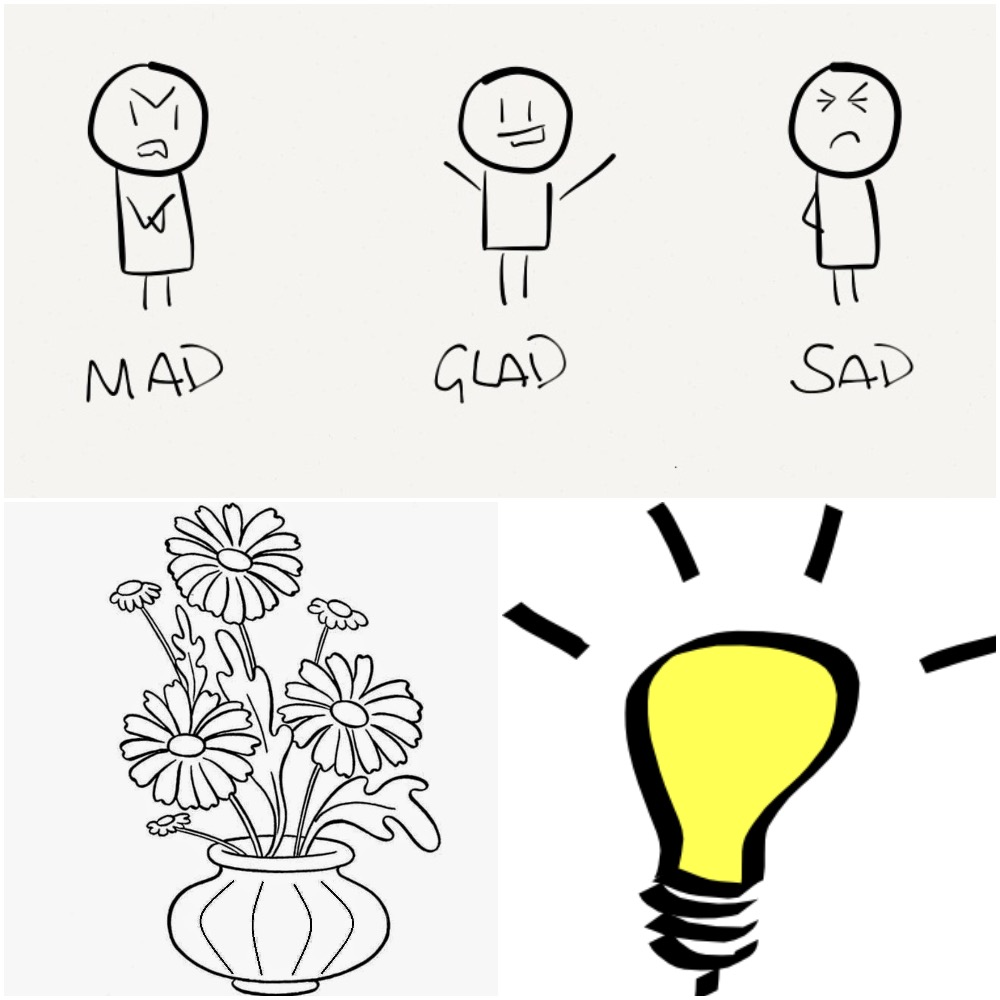
\includegraphics[width=0.5\textwidth]{img/mood}
\end{figure}

Before implementing the game in the team requirements presented in \autoref{tab:mood-req} must be completed and the team needs to be aware how to play the game.

\begin{table}[h]
	\caption{Requirements to start Mood and Improvements game}
	\label{tab:mood-req}
	\begin{tabularx}{\textwidth}{|X|X|}
	\hline
		Target & Retrieve teams mood and maximize solving problems  \\ \hline
		Required			& \begin{enumerate}
		    \item Minimum 3-people scrum team
		    \item Blackboard
		    \item Sticky Notes
		    \item Pencil/Pen
		\end{enumerate}	 \\ \hline
		Time & About \~60 minutes\\ \hline
	\end{tabularx}
\end{table}


\subsection{5L's game}
\label{subch:5LGame}

The second game created, thanks to the collaboration with the Intel Technology Poland teams, is 5L's Game. The activity has not been developed from scratch, there is an existing solution called 4L's \cite{4Ls}, which we have improved, by adding one additional element. The initial version of the game is shown on \autoref{fig:4Ls} and it contained four fields:
\begin{enumerate}
    \item Liked - things that the participants liked about the past iteration, considering project and team.
    \item Learned - things that the team members learned in the past iteration, new language, used new framework or tool, this might also be things not connected to the project like for example while being on a integration with the team the participants learned how to windsurf or make sushi.
    \item Lacked of - things that have been done in the past iteration and you do not want to stop doing them but you have an idea how to do it better, how to improve the action, or just wish that it could be done, for example more efficiently.
    \item Longed for - things that you wish would have been done, for example more attention on code quality, rather than focusing just on the delivery.
\end{enumerate}

\begin{figure}[h]
\caption{4L's} 
\label{fig:4Ls}
\centering
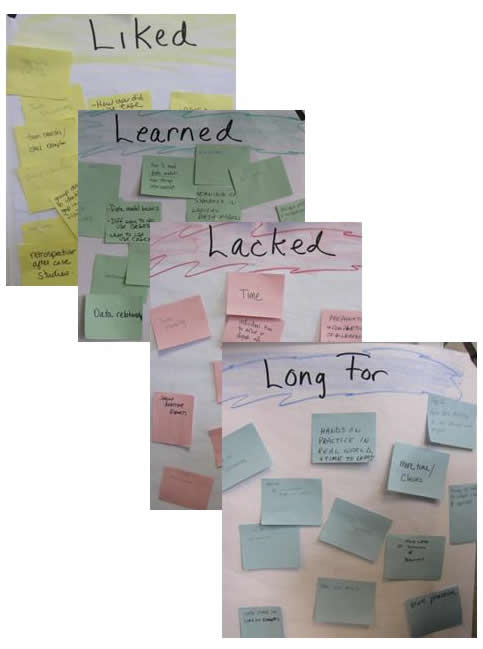
\includegraphics[width=0.5\textwidth]{img/4L}
\end{figure}

While implementing the game the team that we were currently working with (team B) suggested that there should be an area where you can describe things that the team disliked in the past iteration. After a discussion we developed the 5th "L" which was "Loathing". The last "L" included in the initial 4L's game was created in order to retrieve negative feedback from the team and, if possible, improve the area where the problem occurred or even dispose it.

\begin{figure}[h]
\caption{5L's} 
\label{fig:5Ls}
\centering
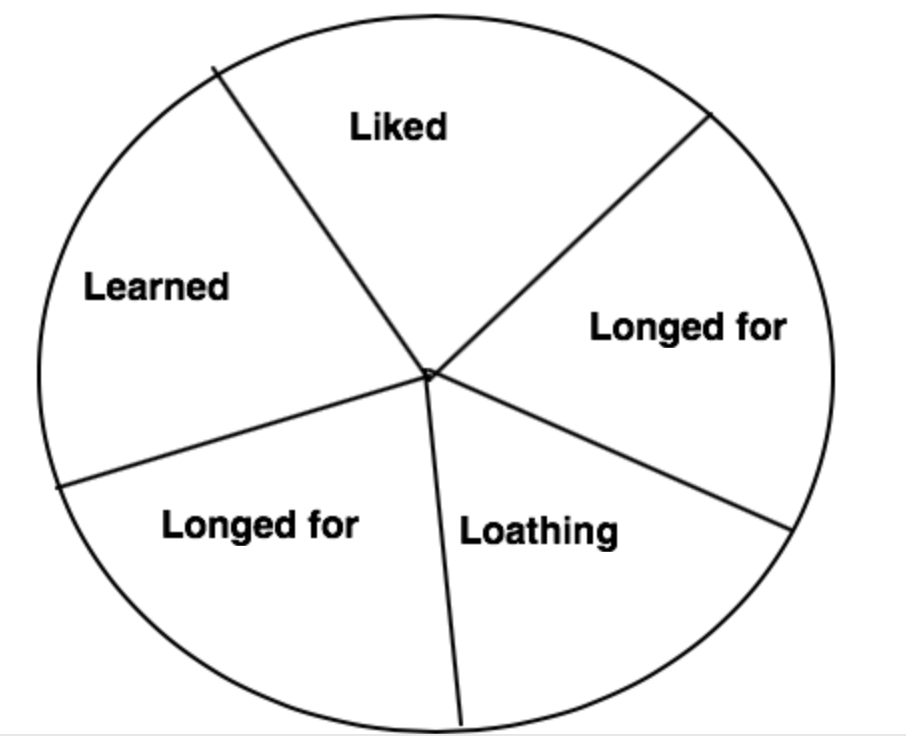
\includegraphics[width=0.5\textwidth]{img/5L}
\end{figure}

\subsection{Candy-Love Game}
Another game, which may be valuable to focus on, is more a team building game rather than solving problems in case of project, but in order to maximize performance and product quality it is advisable to have strong and integrated team \cite{ForbesArticle}. Harvard Business Review claim that "Research shows that when people work with a positive mind-set, performance on nearly every level—productivity, creativity, engagement—improves. Yet happiness is perhaps the most misunderstood driver of performance.". \cite{HarvardArticle} "Candy Love" game integrates team members by letting them speak up and talk about their life beyond work \cite{CandyLoveBibliography}. In order to deploy the game and show it to your team, necessary requirements presented in the \autoref{tab:candylove-req} are needed.

\begin{table}[h]
	\caption{Requirements to start Candy-Love Game}
	\label{tab:candylove-req}
	\begin{tabularx}{\textwidth}{|X|X|}
	\hline
		Target & Increase trust in the team, help people to speak up and get to know each other \\ \hline
		Required			& \begin{enumerate}
		    \item Minimum 3-people scrum team
		    \item Pack of MM's, Skittles or other colourful candies
		    \item Jar for candies
		    \item Meanings of colors (rules)
		\end{enumerate}	 \\ \hline
		Time			& About \~2-4 minutes per person	 \\ \hline
	\end{tabularx}
\end{table}
The participants need to sit at the table, without laptops and other distracting things. One person picks the candy out of the jar and shows it to the team, than checks the candy color meaning. The others need to focus on what the person which picked the candy is talking about. The meanings of the colors are necessary to have in order to properly perform the game, because it's hard to remember all the meanings of the colors, which are as follows: 
\begin{enumerate}
    \item Red - share one thing that you like about your job, this color retrieves positive emotions, especially on people that are not satisfied or happy with what they do.
    \item Yellow - share your life goal that you are working on, this color illustrates others what is important for that person and can inspire.
    \item Green - share your favorite movie or/and book, this shows person from different angle, maybe this might start a conversion later with people that we usually have nothing to talk about.
    \item Purple - share your favorite way of reviving yourself on a regular workday, this color shows what the person thinking about to decrease stress and might be also a great catalyst for a conversation.
    \item Blue - share one stressful thing in work that you wish you could improve, this color shows what stresses person out, maybe someone has a solution that can share, this can also convert a negative thing into a positive.
    \item Orange - share what is your favorite food, maybe later you can share a meal with someone from the team and it is a topic that everyone likes.
\end{enumerate}
The participants should pass the jar to each team member and end the game when all the candies are gone, when all the team members picked one sweet or when the time of the meeting has ended \cite{CandyLoveBibliography}.

\section{Supplementary games}
The techniques that are going to be described in this section are or were probably used by major number of the teams working in information technology, most of them are not aware of its existence and how valuable they are. These approaches are just supplementary games to fundamental ones described in \autoref{s:fundGames}. In order to properly and effectively implement a retrospective meeting the team should chose one of the fundamental games and as an additional value add one or more supplementary game, which may increase number of valuable opinions and feedback from the team. 
\subsection{Anonymous}
\label{subch:anon}

Based on our work in Intel Technology Poland site in Gdańsk and also on Rui Miguel Ferreira \cite{anonymousRetro}, who wrote his article based on Hiren Doshi article, which was posted on Practice Agile Software Development blog, we can discover power of anonymous retrospectives. According to the article \cite{anonymousRetro} no matter how supportive, open and transparent the company is, there will be always individuals that are not eager to share their thoughts with others \cite{dosanddonts}. They suggested the anonymous technique to encourage introvert individuals to also share their point of view on the project. The following model was presented:
\begin{enumerate}
    \item All the participants of the meeting must be involved and take part in this activity.
    \item The data should be anonymous, untraceable to the writer, for example decide that everything will be written using blue pen and capital letters.
    \item Collect the papers into an empty container and mix them.
\end{enumerate}

Using this technique all the team members are comfortable to share their thoughts and opinion without the feeling of shame or embarrassment. According to our research we learned that most of team members do not like retrospective meeting, because they do not like to expose and talk about theirs feelings, opinions and thoughts. Using this approach it might change retrospective into a valuable meeting without forcing participants to talk and what we also discovered once something is told by an extrovert its stops being "taboo" and even introverts add something to discussion \cite{dosanddonts}.

\subsection{Safe Room}
The retrospective is a meeting strictly focused on a team or project and the managers or product owners, if not directly invited to discuss specified problems, should not be present \cite{dosanddonts}. The safe room techniques is also commonly used in such meetings, but as we mentioned before. The retrospective meeting should be always dedicated to the team and theirs issues and the participants should be comfortable to share their thoughts. We already described one approach how to encourage team to speak up, the second technique is to create a "safe room". To put the "safe room" theory into practice, the person, who is leading the meeting should inform the attendants that everything what is said in the room should stay in the room. This technique must be based on assumption that the team trusts each other that whatever is said during the meeting will not be repeated outside the team, it is a non-formal confidentiality agreement. 
\subsection{One-word-retrospective game}
The "One-word-retrospective" is a game that is supposed to help team to deal with feelings. This technique is used to increase the collaboration, respect and improve the understanding in the team \cite{retroBook}. The rules of this supplementary game are as follows:
\begin{enumerate}
    \item Gather the team and ask each participant to tell how does they feel, using just one word, about the past iteration.
    \item Collect all the words, they might be written on sticky-notes using \nameref{subch:anon} technique.
    \item Write all the words on the board, so everyone is able to see them.
    \item Then start to ask the participants why do they feel that way, use the exact words from the board.
    \item List the major issues and confirm them with the team.
\end{enumerate}

The requirement to implement this supplementary game in the team is to have following things \cite{retroBook}:
\begin{enumerate}
    \item Establish trust and openness.
    \item Respect people and their feelings.
    \item Be able to deal with the issues.
\end{enumerate}
The most important thing, not only using one-word-retrospective technique, is to ensure that the team trusts each other, especially because you are dealing with peoples' emotions and feelings. The leader should make sure that in order for people to speak openly, he has to introduce, if necessary, depends on the team, rules like for example the anonymous or/and safe room techniques. 
